\subsection{Justificacion del problema}
Después de la rápida caída del sector del turístico a nivel mundial por causa de la pandemia del 2020, Colombia ha tenido una mejora prometedora a partir del 2022 que inclusive ha impulsado notoriamente el desarrollo de este sector aún más que antes de la pandemia. Esta afirmación está respaldada por los datos estadísticos que la Cámara de Comercio de Bogotá puede ofrecer sobre el sector turístico y su desempeño desde principios de 2019 hasta julio de 2024. Para entender el siguiente gráfico es necesario comprender que el éxito del sector del turismo se mide respecto al porcentaje de cupos que ofrecen para sus actividades y estadías. 

\begin{adjustbox}{
    center,
    caption=[{Porcentaje de ocupación mensual: Total nacional y Bogotá}]{\centering Ocupación mensual Bogotá. Fuente: (DANE, Encuesta mensual de alojamiento EMA (enero 2019 - abril 2024))},
    label={ocupaciónmensualbogota},
    nofloat=figure}

    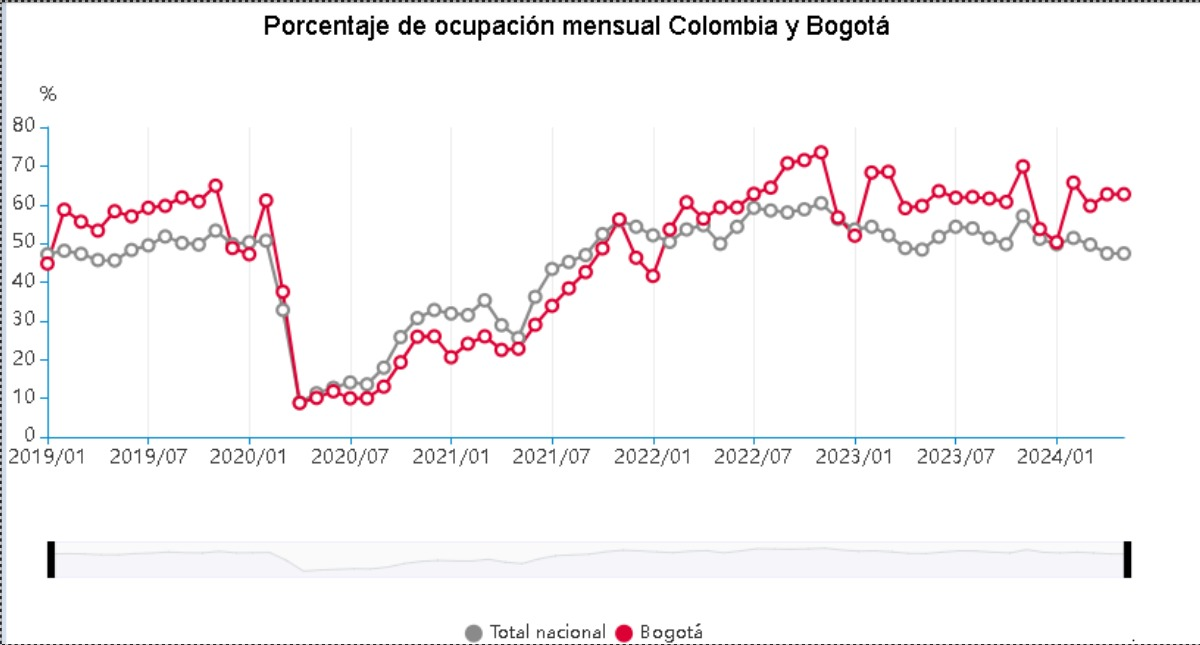
\includegraphics[width=0.2\textwidth]{Content/Images/graficaTurismoBogota.jpeg}

\end{adjustbox}
